\documentclass{beamer}
\mode<presentation>
{
	\usetheme{Madrid}
    
    \definecolor{unisinos}{RGB}{67,40,117}
    \usecolortheme[named=unisinos]{structure}
    
	\usefonttheme{professionalfonts}
    \usebackgroundtemplate{
\includegraphics[width=\paperwidth,height=0.978\paperheight]{template_unisinos}}

 	\beamertemplatenavigationsymbolsempty
 	\setbeamertemplate{footline}
	{
	  \leavevmode%
	  \hbox{%
	  \begin{beamercolorbox}[wd=.12\paperwidth,ht=2.25ex,dp=1ex,center]{author in head/foot}%
	    \usebeamerfont{author in head/foot}\insertshortauthor
	  \end{beamercolorbox}%
	  \begin{beamercolorbox}[wd=.88\paperwidth,ht=2.25ex,dp=1ex,center]{title in head/foot}%
	    \usebeamerfont{title in head/foot}\insertshorttitle\hspace*{3em}
	    \insertframenumber{} / \inserttotalframenumber\hspace*{1ex}
	  \end{beamercolorbox}}%
	  \vskip0pt%
	}
 	\setbeamertemplate{caption}[numbered]
 	\usepackage{caption}

 	\usepackage[brazil]{babel}		% Idioma do documento
	\usepackage{siunitx}
	\usepackage{ragged2e}
	\usepackage{float}
    \usepackage{indentfirst} }
    \usepackage[alf]{abntex2cite}		% Citações padrão ABNT
	\usepackage{color}			% Controle das cores
	\usepackage[T1]{fontenc}		% Selecao de codigos de fonte.
	\usepackage{graphicx}			% Inclusão de gráficos
	\usepackage[utf8]{inputenc}		% Codificacao do documento (conversão automática dos acentos)
	\usepackage{txfonts}			% Fontes virtuais

\title[ Desenvolvimento de um Controlador PID com Auto Sintonia usando Redes Neurais Artificiais e Regressão ...]{Desenvolvimento de um Controlador PID com Auto Sintonia usando Redes Neurais Artificiais e Regressão Não-Linear Robusta para o Controle de Atitude de um Simulador de Satélites com
Rodas de Reação}
\author[Piaia, G. A.]{
	{\fontsize{10}{8}\selectfont \textbf{Aluno:} Guilherme Angelo Piaia} \\
	{\fontsize{10}{8}\selectfont \textbf{Orientador}: Rodrigo Marques de Figueiredo}
}
%\institute[UNISINOS]{UNISINOS - Universidade do Vale do Rio dos Sinos \\ Engenharia de Controle e Automação}

\date{\today}

\begin{document}

%%%%%%%%%%%%%%%%%%%%%%%%%%%%%%%%%%%

\begin{frame}
	\begin{minipage}{1\linewidth}
		\centering
		    \textbf{UNISINOS - Universidade do Vale do Rio dos Sinos} \\ Engenharia de Controle e Automação
	\end{minipage}
	\titlepage
\end{frame}

%%%%%%%%%%%%%%%%%%%%%%%%%%%%%%%%%%%

\begin{frame}{Sumário}
	\tableofcontents
\end{frame}

%%%%%%%%%%%%%%%%%%%%%%%%%%%%%%%%%%%

\section{Introdução}
\begin{frame}{Introdução}
	\begin{itemize}
		\justifying
		\item blablabla blablabla blablabla blablabla 
		\item blablabla blablabla blablabla blablabla 
		\item blablabla blablabla blablabla blablabla 
		\item blablabla blablabla blablabla blablabla 
    \end{itemize}
\end{frame}

%%%%%%%%%%%%%%%%%%%%%%%%%%%%%%%%%%%
\section{Referencial Teórico}
\begin{frame}{Referencial Teórico}
	\begin{itemize}
		\justifying
		\item blablabla blablabla blablabla blablabla 
		\item blablabla blablabla blablabla blablabla 
		\item blablabla blablabla blablabla blablabla 
		\item blablabla blablabla blablabla blablabla 
	\end{itemize}
\end{frame}

%%%%%%%%%%%%%%%%%%%%%%%%%%%%%%%%%%%

\begin{frame}{Referencial Teórico - Dinâmica de um satélite artificial}
    \begin{figure}[HT]
		\begin{center}
		\captionsetup{justification=centering}
        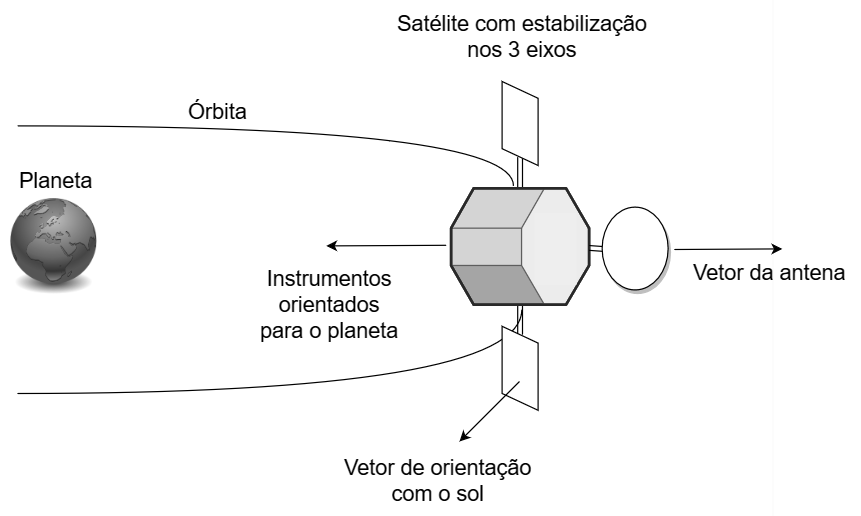
\includegraphics[scale=.42]{../referencial/img/rotational_brown_p256}
        \caption{Movimento de translação de um satélite artificial. \newline
        		 Fonte: Adaptado de \citeonline{Brown2002}.}
		\label{FIG_ADAPTATIVO}
        \end{center}
	\end{figure}
\end{frame}

%%%%%%%%%%%%%%%%%%%%%%%%%%%%%%%%%%%

\begin{frame}{Referencial Teórico - Mecânica de corpo rígido}
	\begin{itemize}
		\justifying
		\item blablabla blablabla blablabla blablabla 
    \end{itemize}

    \begin{equation}
		\vec{\tau}=\dot{\vec{L}}
	\end{equation}
	\begin{equation}\label{eq:iomega}
		\vec{L}=I\vec{\omega}
	\end{equation}
	\begin{equation}\label{iomega}
		\vec{\tau}=I\dot{\vec{\omega}}=I\vec{\alpha}
	\end{equation}
	\begin{equation}
		\dot{\vec{L}}=I\dot{\vec{\omega}}+\vec{\omega}\times I \vec{\omega}
	\end{equation}

\end{frame}

%%%%%%%%%%%%%%%%%%%%%%%%%%%%%%%%%%%

\begin{frame}{Referencial Teórico - Mecânica de corpo rígido}
	\begin{itemize}
		\justifying
		\item blablabla blablabla blablabla blablabla
    \end{itemize}

    \begin{equation}\label{eq:torque}
		\vec{\tau}=I\dot{\vec{\omega}}+\vec{\omega}\times I \vec{\omega}
	\end{equation}
    \begin{equation}
		\begin{bmatrix}\tau_{1}\\\tau_{2}\\\tau_{3}\end{bmatrix}=\begin{bmatrix}A\dot{\omega}_{1}\\B\dot{\omega}_{2}\\C\dot{\omega}_{3}\end{bmatrix}+\begin{bmatrix}\omega_{1}\\\omega_{2}\\\omega_{3}\end{bmatrix}\times\begin{bmatrix}A\omega_{1}\\B\omega_{2}\\C\omega_{3}\end{bmatrix}
	\end{equation}
	\begin{equation}
		\left|\vec{\omega}\right|=\begin{bmatrix}\omega_1\\\omega_2\\\omega_2\end{bmatrix}
	\end{equation}

\end{frame}

%%%%%%%%%%%%%%%%%%%%%%%%%%%%%%%%%%%

\begin{frame}{Referencial Teórico - Mecânica de corpo rígido}
	\begin{itemize}
		\justifying
		\item blablabla blablabla blablabla blablabla 
    \end{itemize}

    \begin{equation}
	  \tau_1=A\dot{\omega_1}-(B-C)\omega_2\omega_3 
	\end{equation}
    \begin{equation}
	  \tau_2=B\dot{\omega_2}-(C-A)\omega_1\omega_3 
	\end{equation}
	\begin{equation}
	  \tau_3=C\dot{\omega_3}-(A-B)\omega_1\omega_2
	\end{equation}
\end{frame}

%%%%%%%%%%%%%%%%%%%%%%%%%%%%%%%%%%%

\begin{frame}{Referencial Teórico - Mecânica de corpo rígido}
	\begin{itemize}
		\justifying
		\item blablabla blablabla blablabla blablabla
    \end{itemize}

	\begin{equation}
	  \dot{\omega_{1}}=\frac{\tau_{1}}{A}+\left(\frac{B-C}{A}\right)\omega_{2}\omega_{3}
	\end{equation}
	\begin{equation}
	  \dot{\omega_{2}}=\frac{\tau_{2}}{B}+\left(\frac{C-A}{B}\right)\omega_{1}\omega_{3}
	\end{equation}
	\begin{equation}
	  \dot{\omega_{3}}=\frac{\tau_{2}}{C}+\left(\frac{A-B}{C}\right)\omega_{1}\omega_{2}
	\end{equation}
\end{frame}

%%%%%%%%%%%%%%%%%%%%%%%%%%%%%%%%%%%

\begin{frame}{Referencial Teórico - Rodas de Reação}
    \begin{figure}[HT]
		\begin{center}
		\captionsetup{justification=centering}
        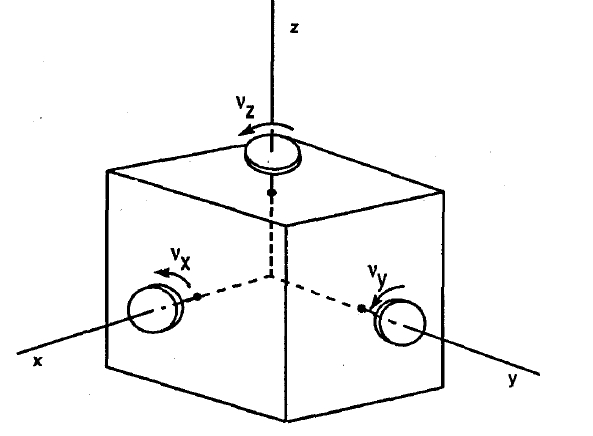
\includegraphics[scale=.42]{../referencial/img/satellite_controlhand_p1306}
        \caption{Representação de um corpo rígido com rodas de reação. \newline
        		 Fonte: Adaptado de \citeonline{Levine1996}.}
		\label{FIG_ADAPTATIVO}
        \end{center}
	\end{figure}
\end{frame}

%%%%%%%%%%%%%%%%%%%%%%%%%%%%%%%%%%%

\begin{frame}{Referencial Teórico - Rodas de Reação}
	\begin{itemize}
		\justifying
		\item blablabla blablabla blablabla blablabla
    \end{itemize}

	\begin{equation}\label{eq:ltot}
		\vec{L}_{total}=\vec{L}_s+\vec{L}_{\omega}=constante 
	\end{equation}

	\begin{equation}
		\vec{L}_s=I\vec{\omega}
	\end{equation}

	\begin{equation}
		\vec {L}_{\omega} =J_{\omega}\vec{\psi}_{\omega}
	\end{equation}

	\begin{equation}\label{eq:torqueedo}
		\vec{\tau}_{\omega}=\dot{\vec{L}}_{\omega}=J_{\omega}\dot{\vec{\psi}}_{\omega}
	\end{equation}
\end{frame}

%%%%%%%%%%%%%%%%%%%%%%%%%%%%%%%%%%%

\begin{frame}{Referencial Teórico - Rodas de Reação}
	\begin{itemize}
		\justifying
		\item blablabla blablabla blablabla blablabla
    \end{itemize}
	\begin{equation}\label{eq:modeloA}
	  \dot{\omega_{1}}=\frac{J_{\omega 1}\dot{\vec{\psi}}_{\omega 1}}{A}+\left(\frac{B-C}{A}\right)\omega_{2}\omega_{3}
	\end{equation}

	\begin{equation}\label{eq:modeloB}
	  \dot{\omega_{2}}=\frac{J_{\omega 2}\dot{\vec{\psi}}_{\omega 2}}{B}+\left(\frac{C-A}{B}\right)\omega_{1}\omega_{3}
	\end{equation}

	\begin{equation}\label{eq:modeloC}
	  \dot{\omega_{3}}=\frac{J_{\omega 3}\dot{\vec{\psi}}_{\omega 3}}{C}+\left(\frac{A-B}{C}\right)\omega_{1}\omega_{2}
	\end{equation}

\end{frame}

%%%%%%%%%%%%%%%%%%%%%%%%%%%%%%%%%%%

\begin{frame}{Referencial Teórico - Controle}
    \begin{figure}[HT]
		\begin{center}
		\captionsetup{justification=centering}
        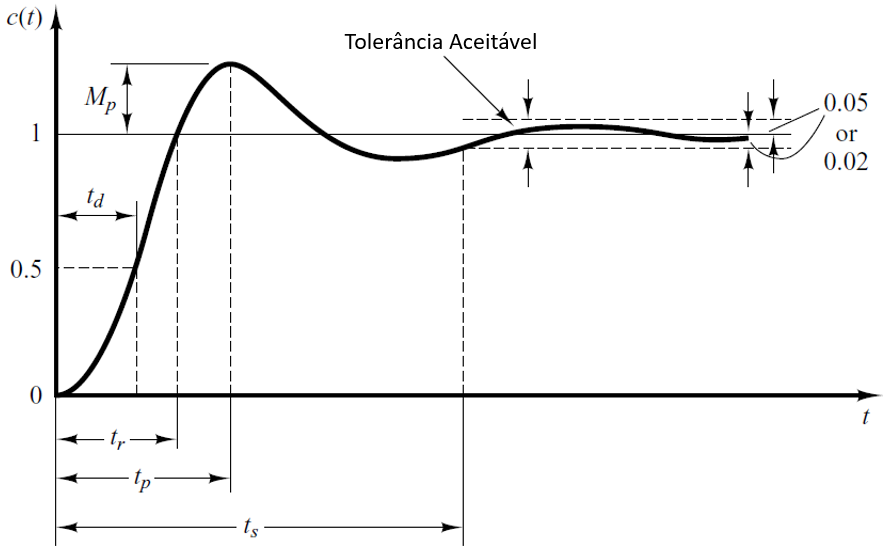
\includegraphics[scale=.35]{../referencial/img/transient_ogata_p170}
        \caption{Parâmetros de uma resposta ao degrau de um sistema de segunda ordem ou superior. \newline
        		 Fonte: Adaptado de \citeonline{Ogata}.}
		\label{FIG_ADAPTATIVO}
        \end{center}
	\end{figure}
\end{frame}

%%%%%%%%%%%%%%%%%%%%%%%%%%%%%%%%%%%

\begin{frame}{Referencial Teórico - Controle}
    \begin{figure}[HT]
		\begin{center}
		\captionsetup{justification=centering}
        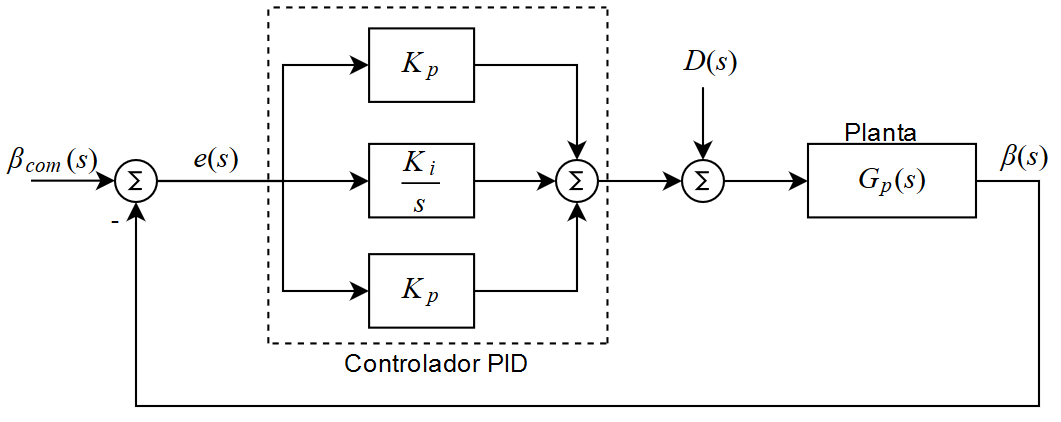
\includegraphics[scale=.45]{../referencial/img/pid_controller_Snider_p35}
        \caption{Representação do modelo paralelo de um controlador PID com distúrbios. \newline
        		 Fonte: Elaborado pelo autor}
		\label{FIG_ADAPTATIVO}
        \end{center}
	\end{figure}
\end{frame}

%%%%%%%%%%%%%%%%%%%%%%%%%%%%%%%%%%%

\begin{frame}{Referencial Teórico - Controle}
    \begin{figure}[HT]
		\begin{center}
		\captionsetup{justification=centering}
        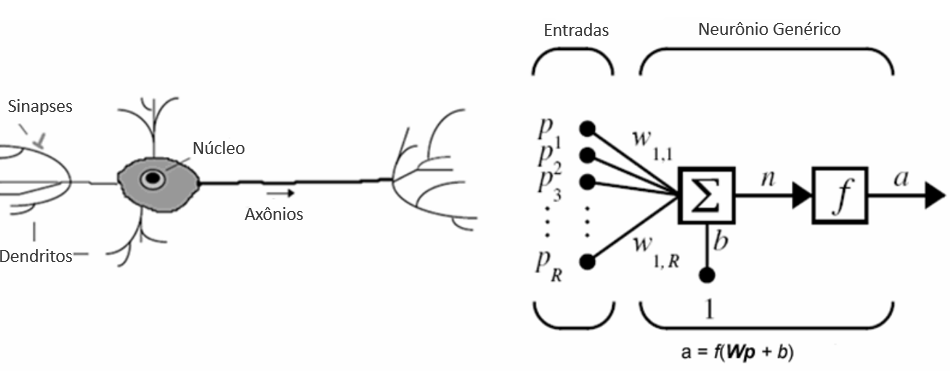
\includegraphics[scale=.35]{../referencial/img/neuronio_unal_p6}
        \caption{Célula de um neurônio natural e modelo matemático respectivo. \newline
        		 Fonte: Adaptado de  \citeonline{Unal2013}.}
		\label{FIG_ADAPTATIVO}
        \end{center}
	\end{figure}
\end{frame}

%%%%%%%%%%%%%%%%%%%%%%%%%%%%%%%%%%%

\begin{frame}{Referencial Teórico - Estado da Arte}
    \begin{figure}[HT]
		\begin{center}
		\captionsetup{justification=centering}
        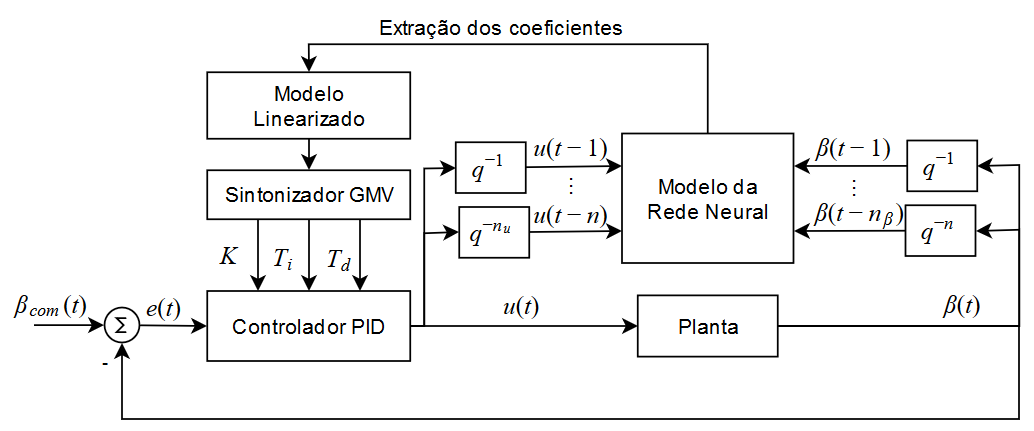
\includegraphics[scale=.42]{../referencial/img/pid_neural_chen_p212}
        \caption{Controlador PID com rede neural. \newline
        		 Fonte: Adaptado de \citeonline{Chen2004}.}
		\label{FIG_ADAPTATIVO}
        \end{center}
	\end{figure}
\end{frame}

%%%%%%%%%%%%%%%%%%%%%%%%%%%%%%%%%%%

\section{Metodologia}
\begin{frame}{Metodologia}
	\begin{itemize}
		\justifying
		\item blablabla blablabla blablabla blablabla 
		\item blablabla blablabla blablabla blablabla 
		\item blablabla blablabla blablabla blablabla 
		\item blablabla blablabla blablabla blablabla 
    \end{itemize}
\end{frame}

%%%%%%%%%%%%%%%%%%%%%%%%%%%%%%%%%%%

\begin{frame}{Metodologia - Hardware}
    \begin{figure}[HT]
		\begin{center}
		\captionsetup{justification=centering}
        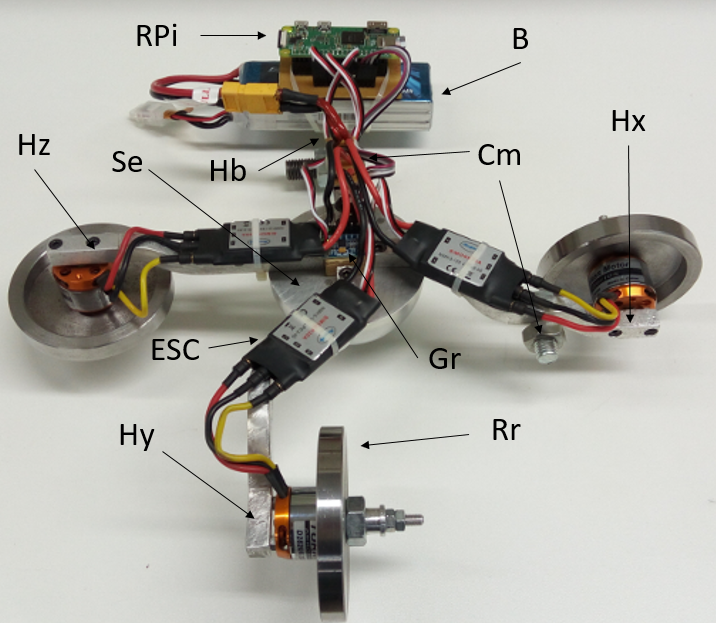
\includegraphics[scale=.35]{../metodologia/img/corpo_real}
        \caption{Corpo do simulador de satélites prototipado. \newline
        		 Fonte: Elaborado pelo autor.}
		\label{FIG_ADAPTATIVO}
        \end{center}
	\end{figure}
\end{frame}

%%%%%%%%%%%%%%%%%%%%%%%%%%%%%%%%%%%

\begin{frame}{Metodologia - Hardware}
    \begin{figure}[HT]
		\begin{center}
		\captionsetup{justification=centering}
        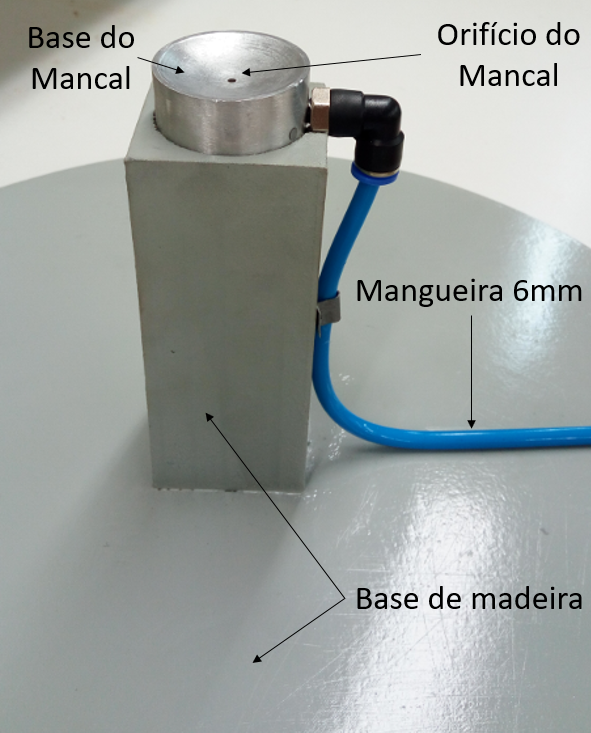
\includegraphics[scale=.3]{../metodologia/img/base_real}
        \caption{Base do simulador de satélites prototipado. \newline
        		 Fonte: Elaborado pelo autor.}
		\label{FIG_ADAPTATIVO}
        \end{center}
	\end{figure}
\end{frame}

%%%%%%%%%%%%%%%%%%%%%%%%%%%%%%%%%%%

\begin{frame}{Metodologia - Hardware}
    \begin{figure}[HT]
		\begin{center}
		\captionsetup{justification=centering}
        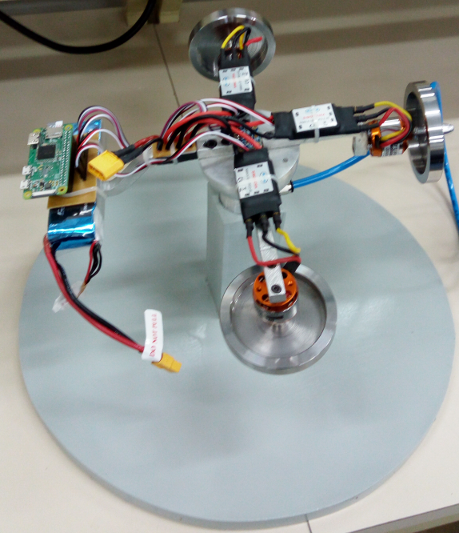
\includegraphics[scale=.3]{../metodologia/img/simulador_real}
        \caption{Simulador de satélites prototipado. \newline
        		 Fonte: Elaborado pelo autor.}
		\label{FIG_ADAPTATIVO}
        \end{center}
	\end{figure}
\end{frame}

%%%%%%%%%%%%%%%%%%%%%%%%%%%%%%%%%%%

\begin{frame}{Metodologia - Sistema de controle}

\begin{columns}
    \begin{column}{0.40\textwidth}
        \begin{figure}[HT]
		\begin{center}
		\captionsetup{justification=centering}
        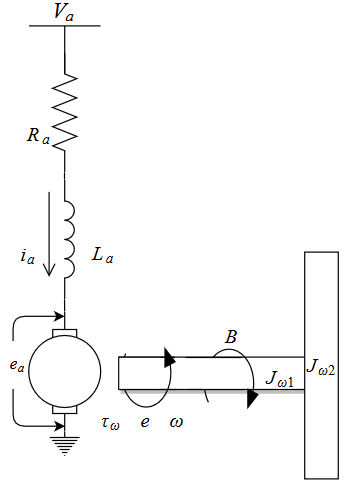
\includegraphics[scale=.4]{../metodologia/img/modelo_motor_dc}
        \caption{Modelo do motor DC. \newline
        		 Fonte: Elaborado pelo autor.}
		\label{FIG_ADAPTATIVO}
        \end{center}
	\end{figure}
    \end{column}
    \begin{column}{0.60\textwidth}
    \begin{itemize}
    	\justifying
    	\item blablabla blablabla blablabla blablabla
    \end{itemize}


	\begin{equation}\label{eq:motor_accel}
	  	\frac{\dot{\omega}(s)}{V_a(s)} = \frac{K_wK_t s}{(R_a+ Las)(Js+B)+K_wK_t}  
	\end{equation}
    \end{column}
\end{columns}
\end{frame}

%%%%%%%%%%%%%%%%%%%%%%%%%%%%%%%%%%%

\begin{frame}{Metodologia - Sistema de controle}
    \begin{figure}[HT]
		\begin{center}
		\captionsetup{justification=centering}
        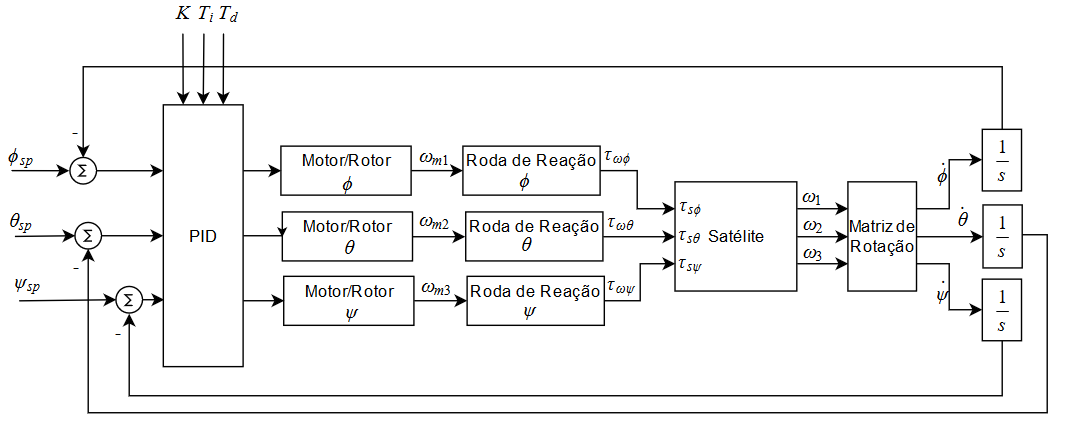
\includegraphics[scale=.42]{../metodologia/img/modelo_satelite_pid}
        \caption{Modelo em malha fechada com um controlador PID. \newline
        		 Fonte: Elaborado pelo autor.}
		\label{FIG_ADAPTATIVO}
        \end{center}
	\end{figure}
\end{frame}

%%%%%%%%%%%%%%%%%%%%%%%%%%%%%%%%%%%

\begin{frame}{Metodologia - Sistema de controle}
    \begin{figure}[HT]
		\begin{center}
		\captionsetup{justification=centering}
        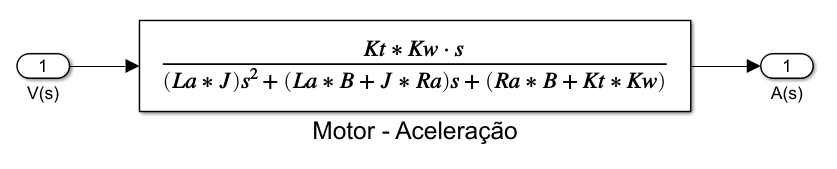
\includegraphics[scale=.25]{../metodologia/img/modelo_satelite_motor}
        \caption{Função de transferência dos motores. \newline
        		 Fonte: Elaborado pelo autor.}
		\label{FIG_ADAPTATIVO}
        \end{center}
	\end{figure}

    \begin{figure}[HT]
		\begin{center}
		\captionsetup{justification=centering}
        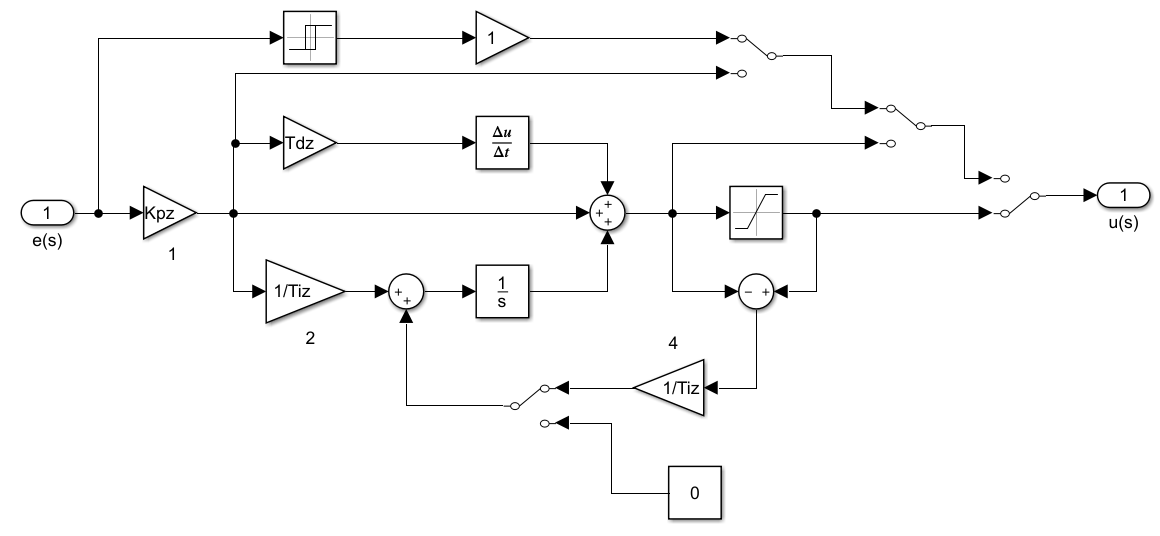
\includegraphics[scale=.25]{../metodologia/img/matlab_pid_antiwindup}
        \caption{Digrama de blocos do controlador PID com Anti-Windup. \newline
        		 Fonte: Elaborado pelo autor.}
		\label{FIG_ADAPTATIVO}
        \end{center}
	\end{figure}
\end{frame}

%%%%%%%%%%%%%%%%%%%%%%%%%%%%%%%%%%%

\begin{frame}{Metodologia - Software}
    \begin{figure}[HT]
		\begin{center}
		\captionsetup{justification=centering}
        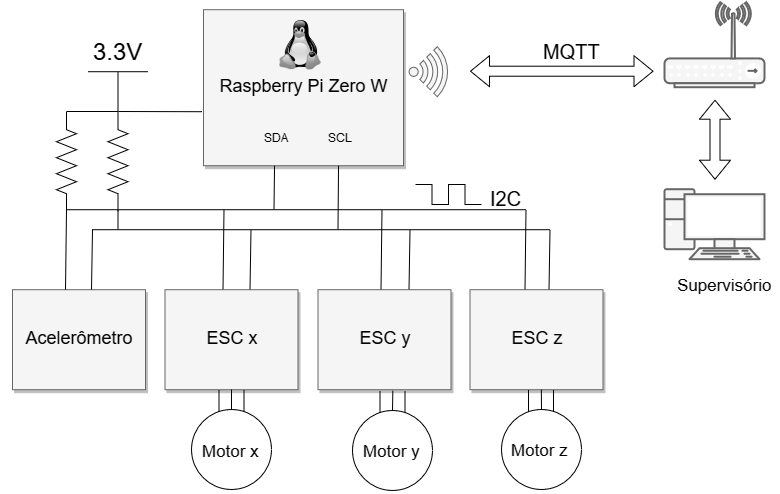
\includegraphics[scale=.45]{../metodologia/img/comunicacao_projeto}
        \caption{Representação geral do sistema. \newline
        		 Fonte: Elaborado pelo autor.}
		\label{FIG_ADAPTATIVO}
        \end{center}
	\end{figure}
\end{frame}

%%%%%%%%%%%%%%%%%%%%%%%%%%%%%%%%%%%

\begin{frame}{Metodologia - Software}
    \begin{figure}[HT]
		\begin{center}
		\captionsetup{justification=centering}
        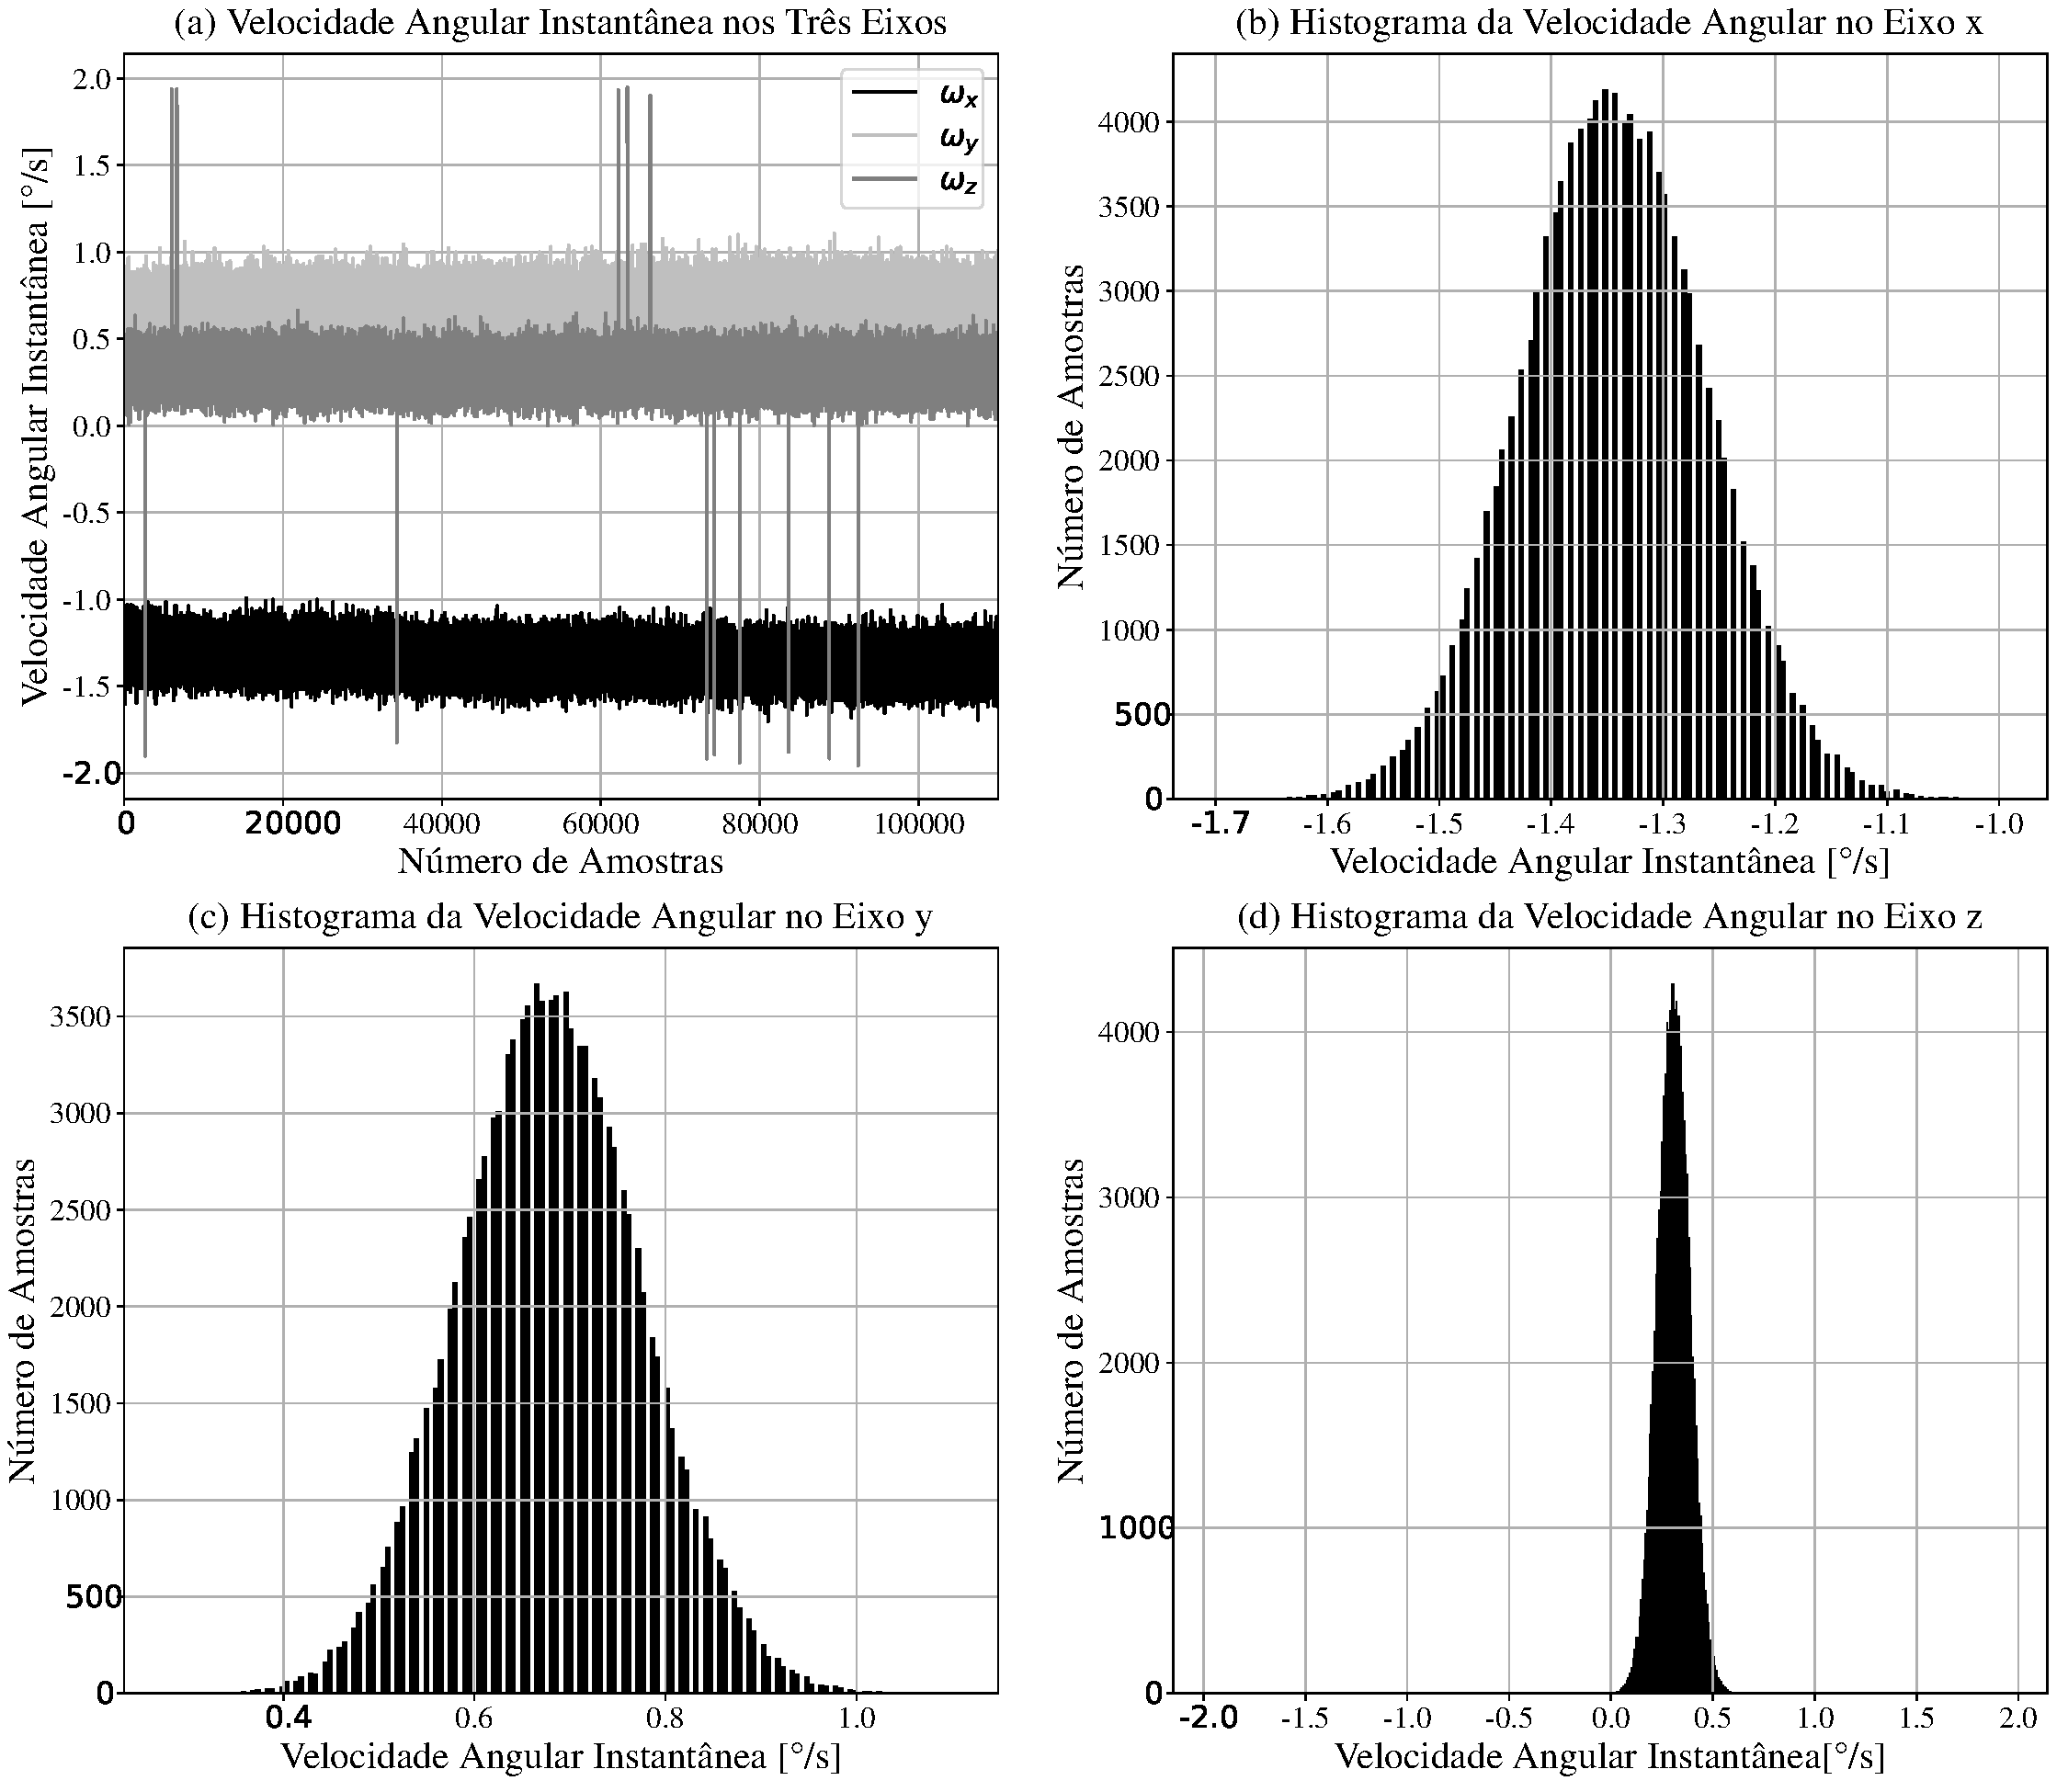
\includegraphics[scale=.17]{../metodologia/img/bias_correction}
        \caption{Características dos sinais amostrados pelo giroscópio. \newline
        		 Fonte: Elaborado pelo autor.}
		\label{FIG_ADAPTATIVO}
        \end{center}
	\end{figure}
\end{frame}

%%%%%%%%%%%%%%%%%%%%%%%%%%%%%%%%%%%

\section{Análise dos Resultados}
\begin{frame}{Análise dos Resultados - Treinamento da RNA}
	\begin{itemize}
		\justifying
		\item blablabla blablabla blablabla blablabla 
		\item blablabla blablabla blablabla blablabla 
		\item blablabla blablabla blablabla blablabla 
		\item blablabla blablabla blablabla blablabla 
	\end{itemize}
\end{frame}

%%%%%%%%%%%%%%%%%%%%%%%%%%%%%%%%%%%

\begin{frame}{Análise dos Resultados - Treinamento da RNA}
     \begin{figure}[HT]
		\begin{center}
		\captionsetup{justification=centering}
        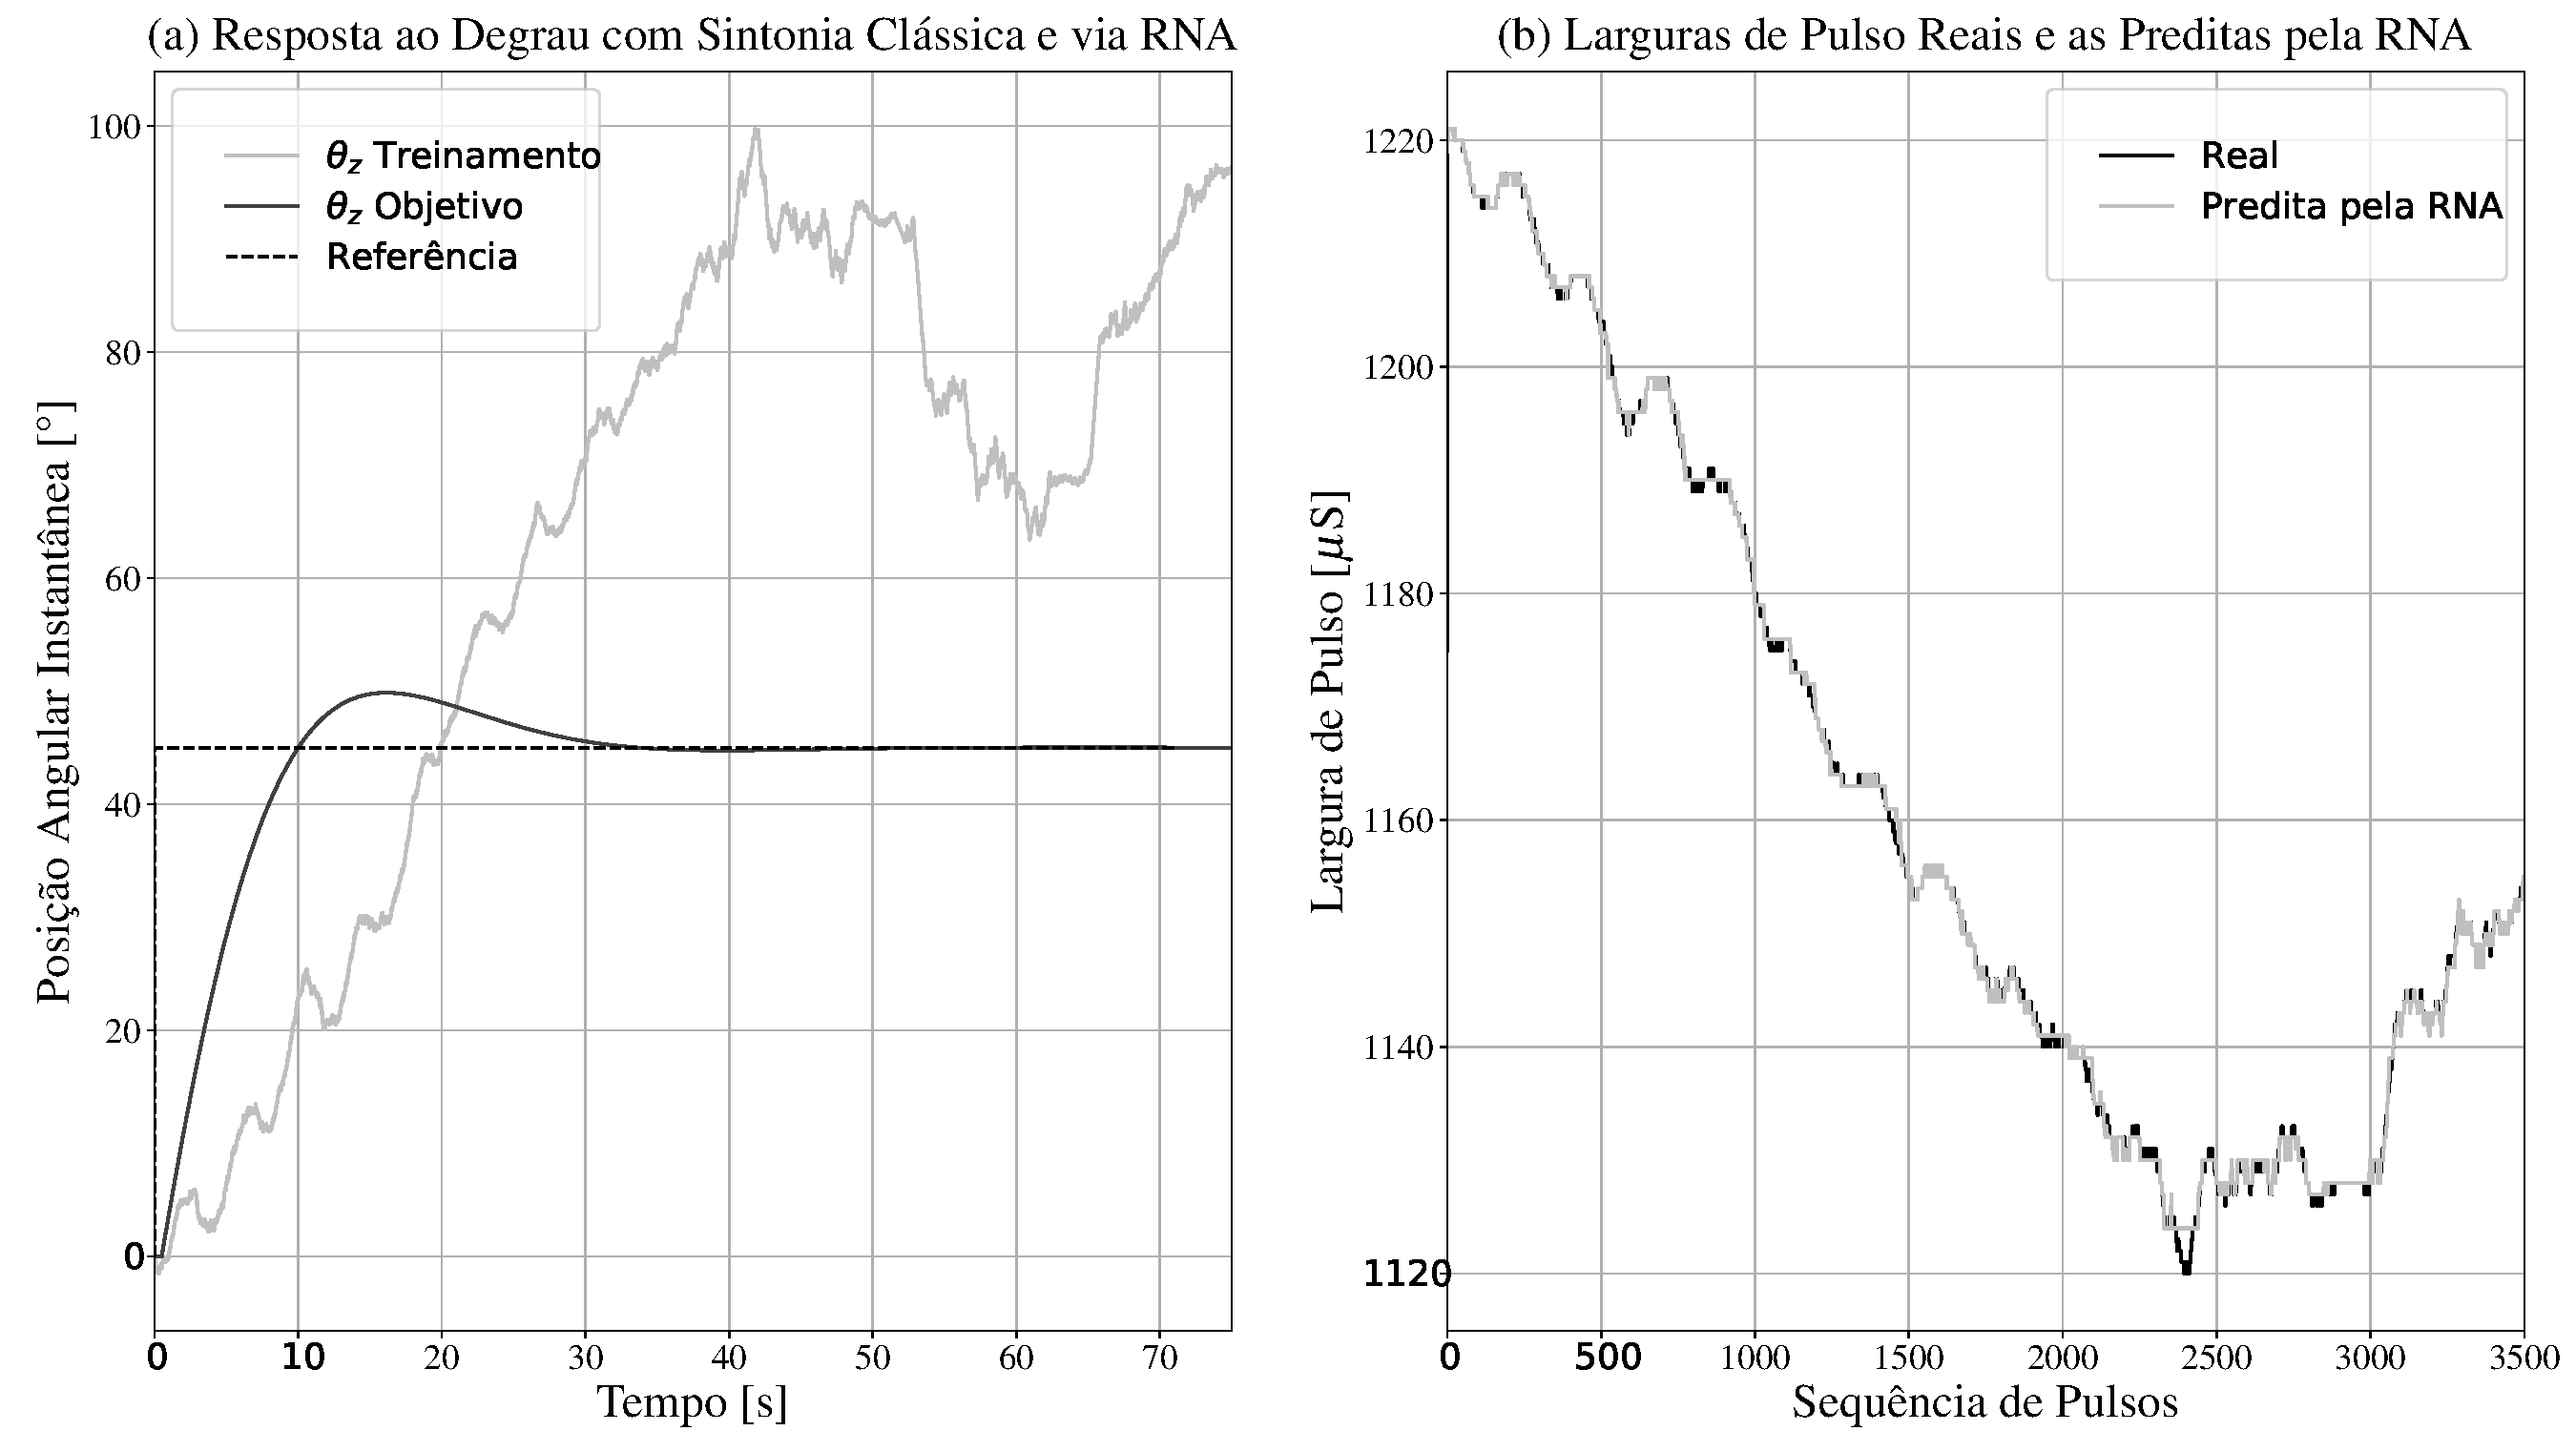
\includegraphics[scale=.22]{../resultados/img/neural_output}
        \caption{Saída da RNA treinada e o sinal real. \newline
        		 Fonte: Elaborado pelo autor.}
		\label{FIG_ADAPTATIVO}
        \end{center}
	\end{figure}
\end{frame}

%%%%%%%%%%%%%%%%%%%%%%%%%%%%%%%%%%%

\begin{frame}{Análise dos Resultados - Método do Relé}
     \begin{figure}[HT]
		\begin{center}
		\captionsetup{justification=centering}
        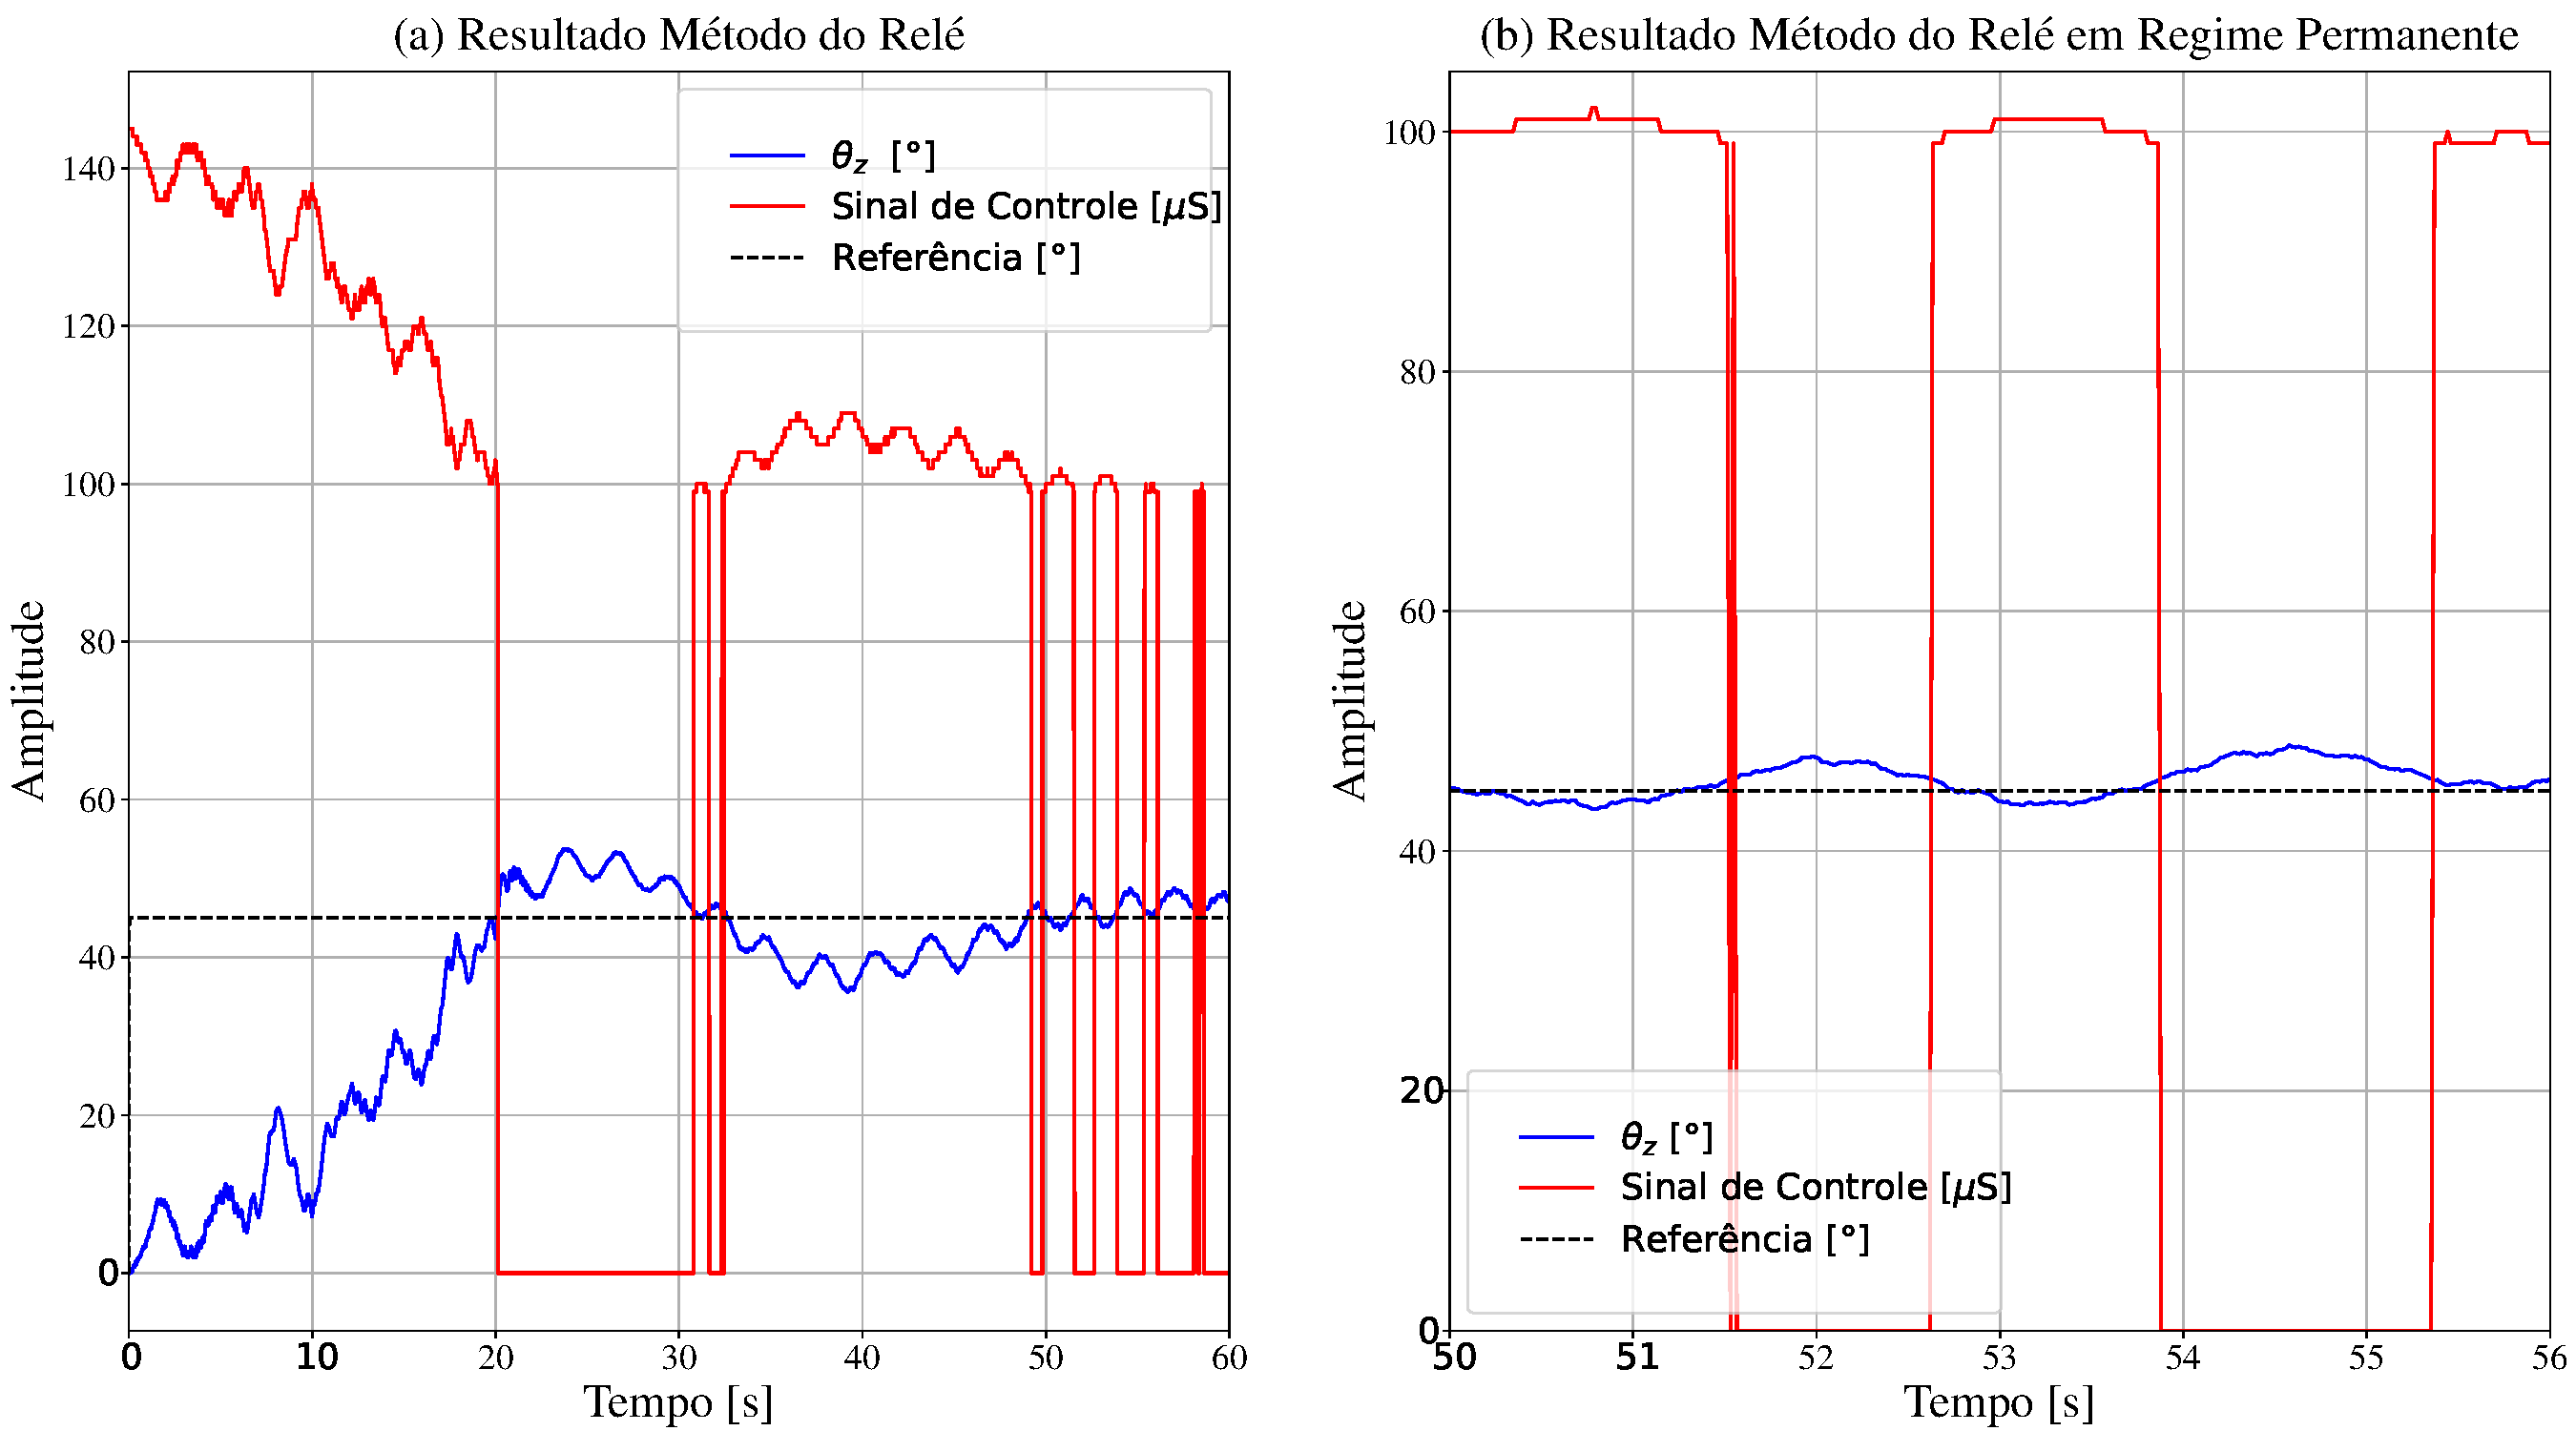
\includegraphics[scale=.22]{../resultados/img/relay}
        \caption{Resultados do método do relé. \newline
        		 Fonte: Elaborado pelo autor.}
		\label{FIG_ADAPTATIVO}
        \end{center}
	\end{figure}
\end{frame}

%%%%%%%%%%%%%%%%%%%%%%%%%%%%%%%%%%%

\begin{frame}{Análise dos Resultados - Respostas ao degrau}
     \begin{figure}[HT]
		\begin{center}
		\captionsetup{justification=centering}
        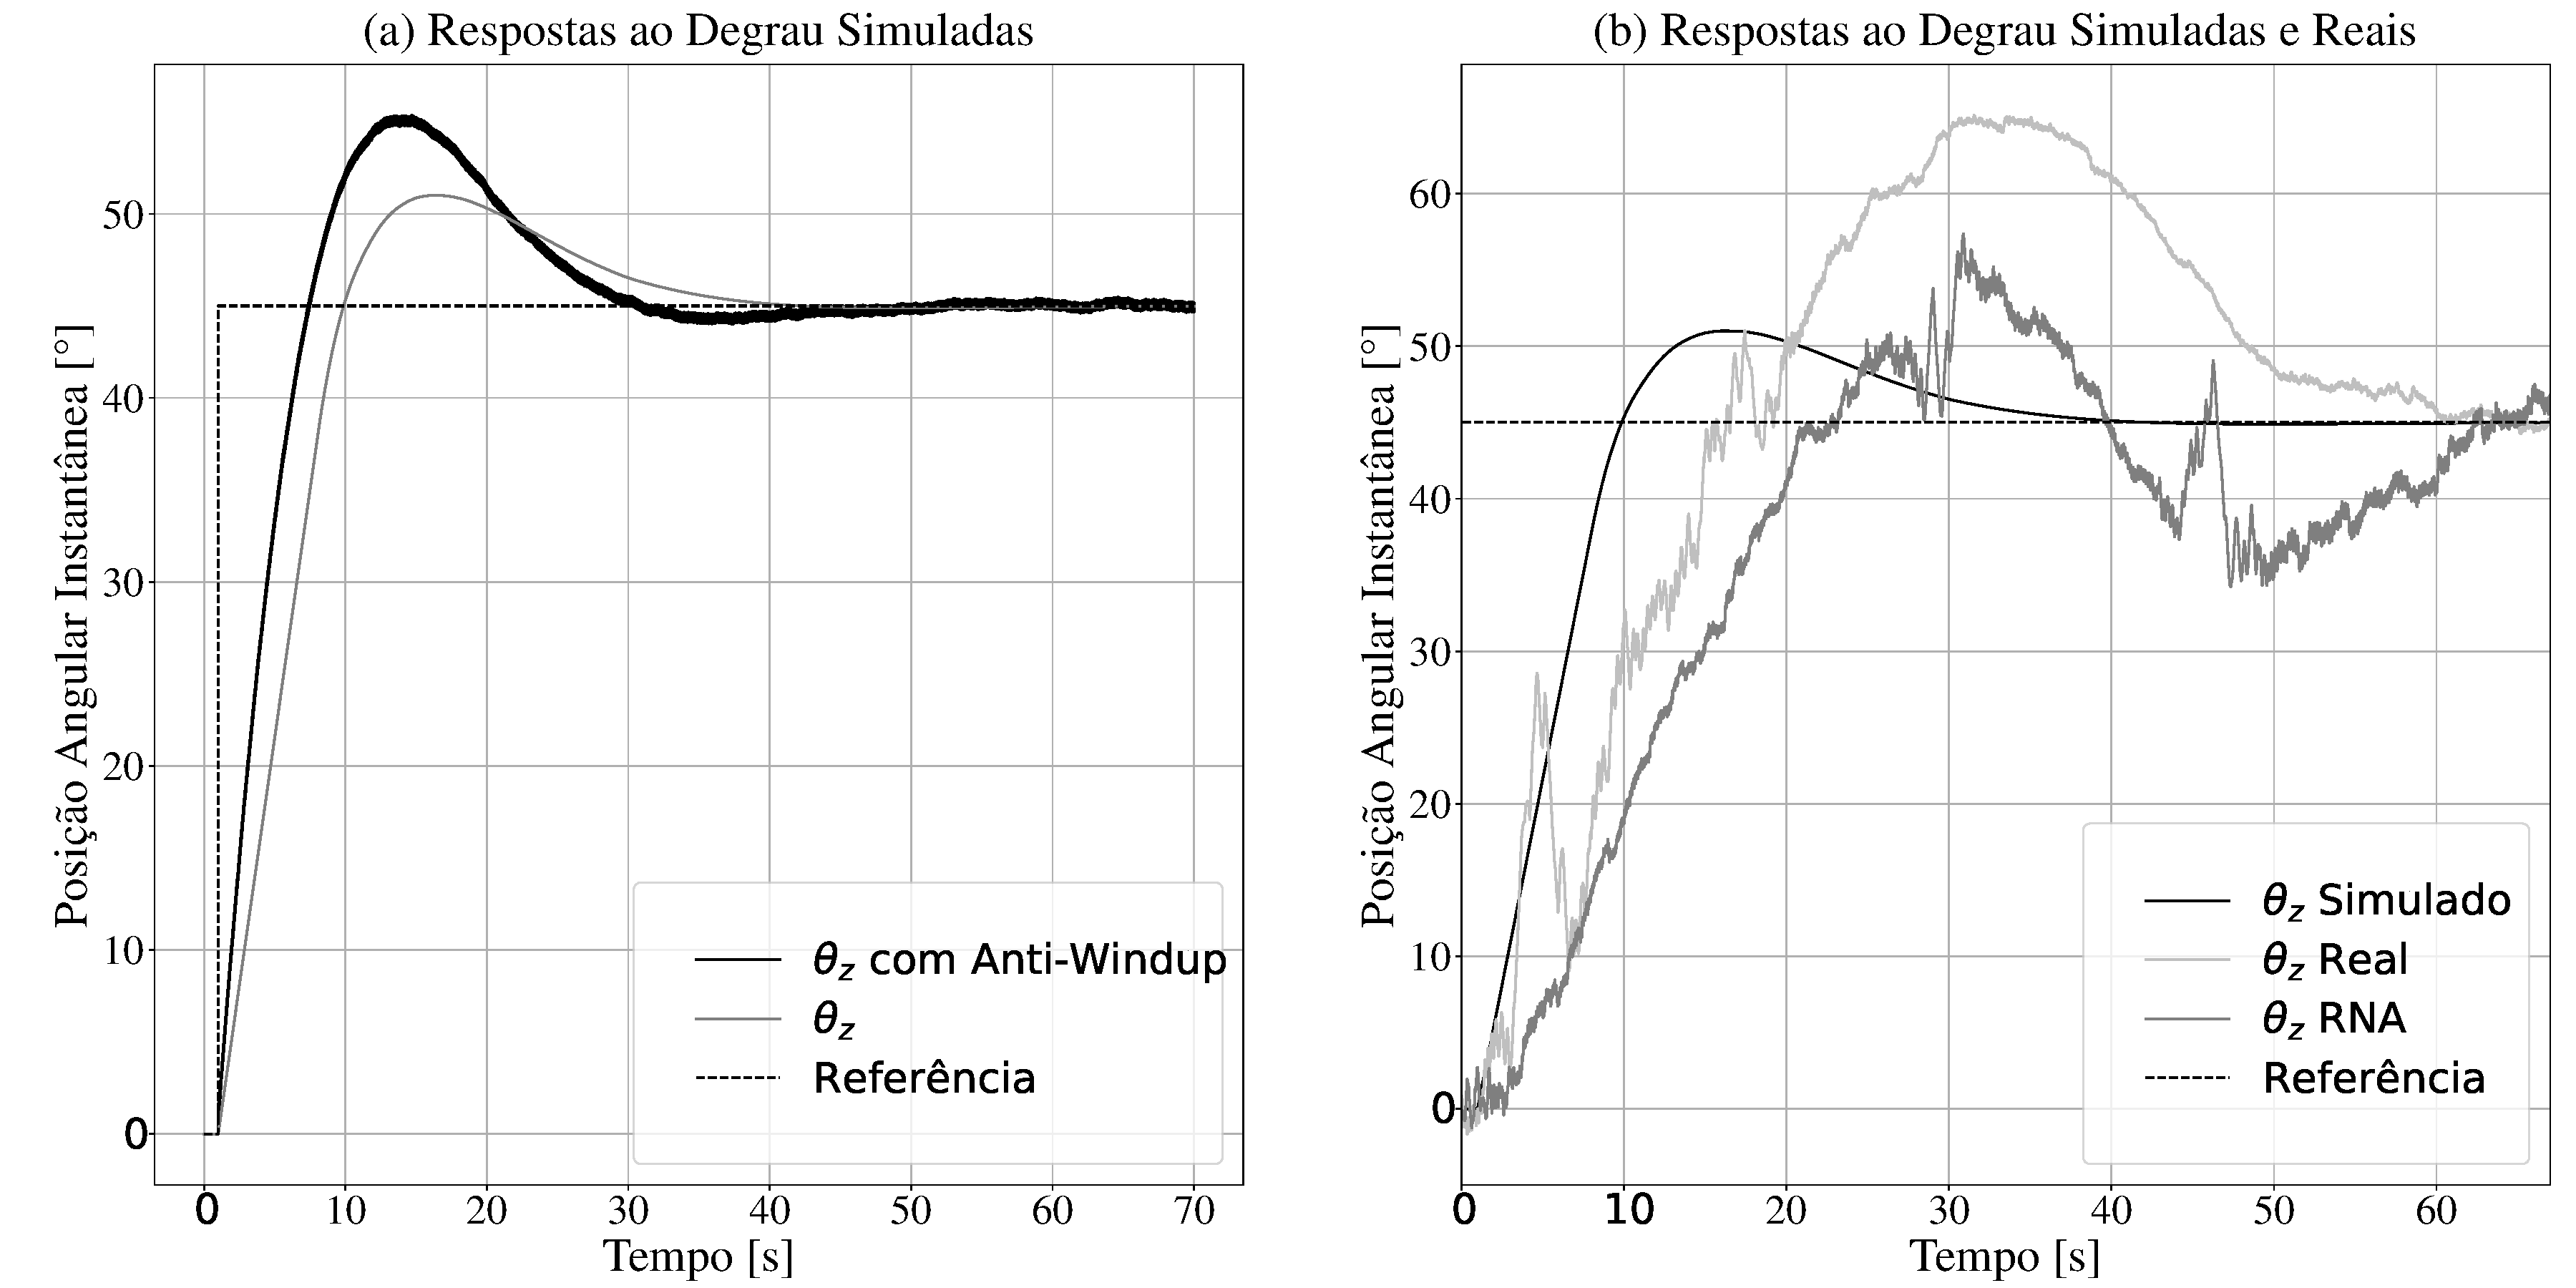
\includegraphics[scale=.18]{../resultados/img/pid_result}
        \caption{Respostas ao degrau com sintonia via método do relé. \newline
        		 Fonte: Elaborado pelo autor.}
		\label{FIG_ADAPTATIVO}
        \end{center}
	\end{figure}
\end{frame}

%%%%%%%%%%%%%%%%%%%%%%%%%%%%%%%%%%%

\begin{frame}{Análise dos Resultados - Respostas ao degrau}
     \begin{figure}[HT]
		\begin{center}
		\captionsetup{justification=centering}
        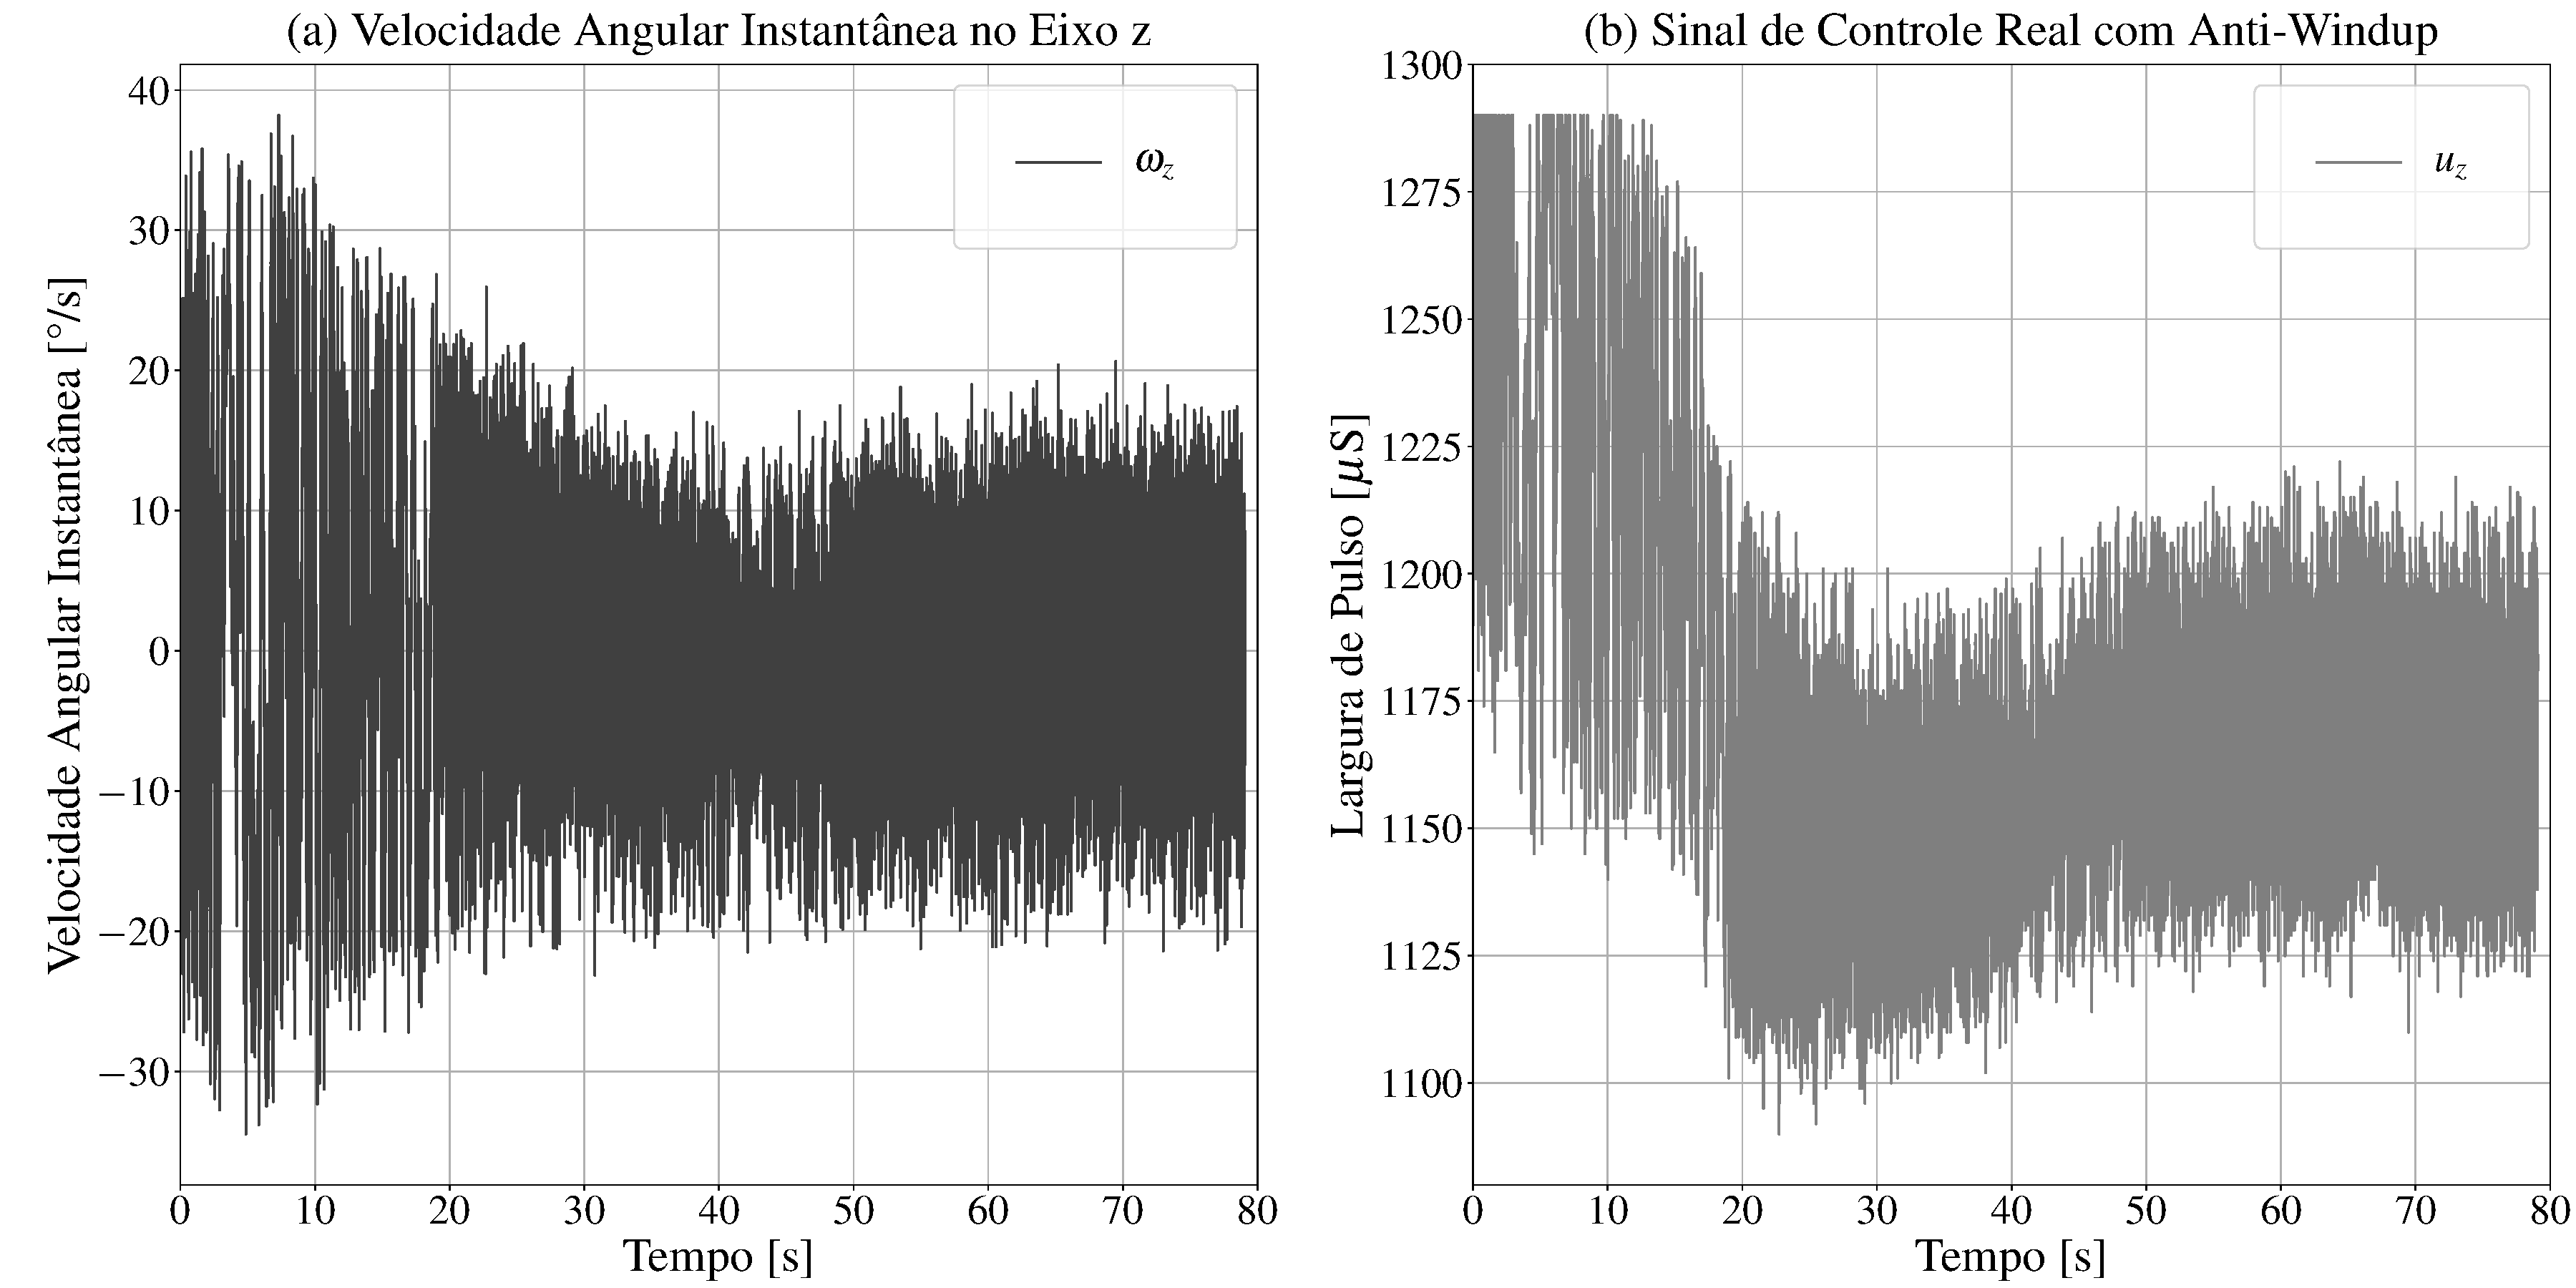
\includegraphics[scale=.18]{../resultados/img/pid_result_controller}
        \caption{Velocidade angular instantânea e sinal de controle. \newline
        		 Fonte: Elaborado pelo autor.}
		\label{FIG_ADAPTATIVO}
        \end{center}
	\end{figure}
\end{frame}

%%%%%%%%%%%%%%%%%%%%%%%%%%%%%%%%%%%

\section{Conclusão}
	\begin{frame}{Conclusão}
    \begin{itemize}
        	\justifying
			\item blablabla blablabla blablabla blablabla
			\item blablabla blablabla blablabla blablabla 
			\item blablabla blablabla blablabla blablabla 
			\item blablabla blablabla blablabla blablabla 
		\end{itemize}
\end{frame}

%%%%%%%%%%%%%%%%%%%%%%%%%%%%%%%%%%%

\begin{frame}{Conclusão - Trabalhos futuros}
    \begin{itemize}
        \justifying
		\item blablabla blablabla blablabla blablabla 
		\item blablabla blablabla blablabla blablabla 
		\item blablabla blablabla blablabla blablabla 
		\item blablabla blablabla blablabla blablabla 
		\end{itemize}
\end{frame}

%%%%%%%%%%%%%%%%%%%%%%%%%%%%%%%%%%%

\section{Referências}
\begin{frame}{Referências Bibliográficas}
	\bibliography{../referencial/references}
\end{frame}
        
%%%%%%%%%%%%%%%%%%%%%%%%%%%%%%%%%%%

\begin{frame}{Agradecimentos}
	\begin{itemize}
        \justifying
        	\item Ao meu orientador Rodrigo Marques de Figueiredo. 
        	\item Aos professores Walter Andrey Fontana e Dilson Jose Aguiar de Souza.
			\item Aos laboratoristas dos laboratórios da Eng. Mecânica.
			\item Aos laboratoristas dos laboratórios da Eng. Elétrica.
			\item Aos demais amigos e familiares que, que de alguma forma, ajudaram na elaboração desse trabalho.  
		\end{itemize}
	\end{frame}

%%%%%%%%%%%%%%%%%%%%%%%%%%%%%%%%%%%

\begin{frame}{Agradecimentos}
		\begin{center}
			{\Huge Obrigado pela Atenção!}
		\end{center}
\end{frame}

\end{document}